\documentclass{amsart}
\usepackage[margin=3cm]{geometry}                % See geometry.pdf to learn the layout options. There are lots.
\geometry{letterpaper}                   % ... or a4paper or a5paper or ...
%\geometry{landscape}                % Activate for for rotated page geometry
\usepackage[parfill]{parskip}    % Activate to begin paragraphs with an empty line rather than an indent
\usepackage{float}
\usepackage{graphicx}
\usepackage{amssymb}
\usepackage{epstopdf}
\usepackage{siunitx}
\usepackage{subcaption}
\usepackage{setspace}
\setstretch{1.3}

\DeclareGraphicsRule{.tif}{png}{.png}{`convert #1 `dirname #1`/`basename #1 .tif`.png}

\title{Frank-Hertz Experiment}
\author{Caspar \textsc{Lant}} % Author name

\date{February 9, 2016} % Date for the report

\begin{document}

\bigskip

\maketitle % Insert the title, author and date
\begin{center}

Intermediate Experimental Physics II\\
\vspace{1.5cm}

\begin{tabular}{l r}

Section: & 002\\
\\
Date Performed: & February 2, 2016 \\ % Date the experiment was performed
Date Due: & Februrary 9, 2016\\
\\
Partner: & Niel Saddeler \\ % Partner names
Professor: & Prof. Andrew Kent\\
Instructor: & David Mykytyn Esquire % Instructor/supervisor
\end{tabular}
\end{center}
\vspace{50mm}
\pagebreak

\paragraph{\textbf{The Objective} of this week's experiment was to honor and replicate the historic Franck-Hertz experiment, which first illustrated the discrete nature of atomic energy levels, and gave us a glimpse into quantum mechanics.}

\section{Theoretical Background/ Abstract}
\paragraph{Just over a century ago, Danish physicsist and renowned goalkeeper Niels Bohr postulated that the energy levels available to the electron in the hydrogen atom were discrete and of a quantum nature. These energy levels are seperated by a potential of 4.9 electron volts. It was James Franck and Gustav Hertz who first validated Bohr's predictions through experiment. The researchers developed a vaccuum tube containing a small quantity of mercury, and anode, a cathode, and a metallic screen. The cathode was to be heated up to a temperature above the vaporization point of mecury (which isn't very high), and subjected to an increasing voltage. The free electrons in the tube would become energized and occasionally collide with the vaporized mercury atoms. Frank and Hertz noticed that the electrons could only lose a specific amount of kinetic energy from each collision\--- yup, 4.9 electron volts, which was detected by measuring the voltages of the screen. This discovery, needless to say, earned them a Nobel prize.}

\section{Experimental Procedure}
\begin{enumerate}
\item Carefully remove the extremely expensive tube from its bubble wrap cocoon.
\item Delicately slot the tube into the socket of the supplied cable, and place it in the oven.
\item Attach the other end of the cable to the propriety apparatus
\item Do not break the tube! It's expensive!
\item Turn on the measurement apparatus, as well as the oscilloscope.
\item Set the switch to reset.
\item Set the value of $U_3$ to 1.5V.
\item Wait about 20 minutes for the Frank-Hertz tube to reach its operating temperature $\vartheta_s = 188^{\circ}$.
\item Turn the largest dial to the sawtooth position, and dial $U_1$ and $U_3$ such that the function displayed on the 'scope approximates the curve found on the last page of the instruction packet.
\item Set up DataStudio with voltage sensors A and B connected to the oscilloscope inputs.
\item Create a graph of voltage B vs. voltage A.
\item Send a single sawtooth wave into the DataStudio interface by using the dial on the Frank-Hertz power supply. You should see a more detailed view of the initial oscilloscope trace on your DataStudio display.
\item Calculate the distance between two peaks using DataStudio's wonderfully intuitive interface! This should come to about 4.9V; the value postulated by Niels Bohr well before your grandparents were alive.
\item You're done! Don't break the tube!
\end{enumerate}

\section{Graphs and Calculations}

\begin{figure}[H]
    \begin{minipage}{0.65\textwidth}
        \centering
        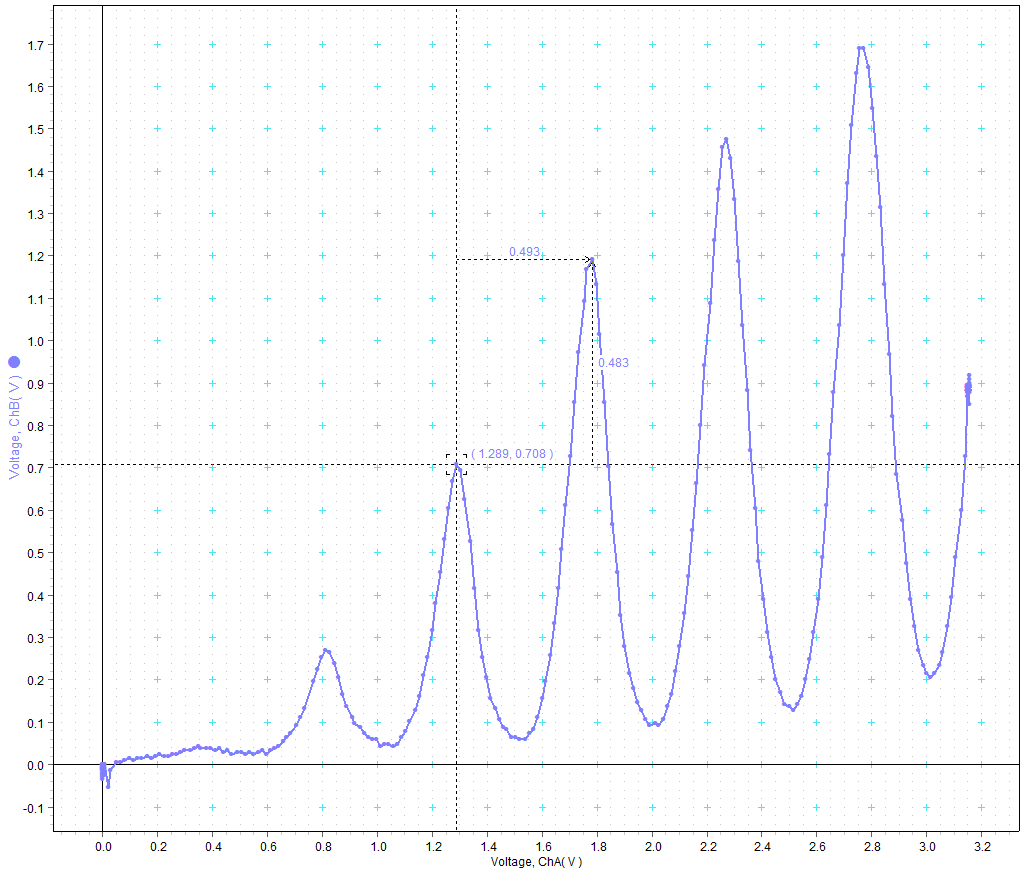
\includegraphics[width=0.9\textwidth]{graph.png}
        \caption{Discrete Energy Levels at Intervals of 4.9V}
    \end{minipage}
    %
    \begin{minipage}{0.3\textwidth}
        This figure demonstrates the quantum nature of electrons. The electrons which fly through the vaccum tube can only sustain kinetic energies of integer multiples of 4.9 electron volts. The y-axis in this figure corresponds to the voltage of the grid, where the x-axis corresponds to the anode voltage. The kinetic energy lost after inelastic collisions between free electrons and mercury atoms is accounted for by light emmission, which isn't seen because lies outside the visible spectrum. Aside from that, the tube is in an oven, which is opaque.
        \vspace{0.23cm}
    \end{minipage}
\end{figure}

\begin{figure}[H]
    \begin{minipage}{0.66\textwidth}
        \centering
        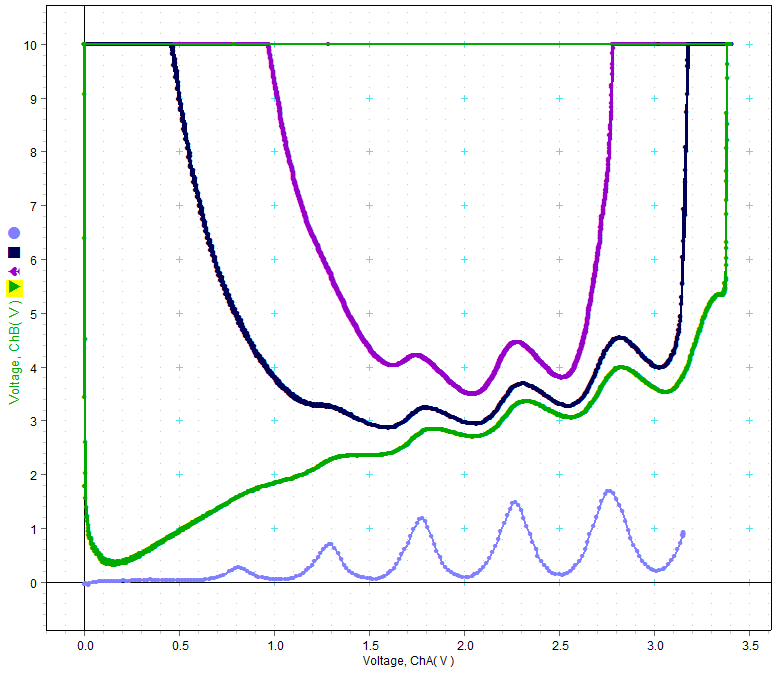
\includegraphics[width=0.9\textwidth]{saturation.png}
        \caption{Saturation of Oscilloscope Trace}
    \end{minipage}
    %
    \begin{minipage}{0.30\textwidth}
        This figure demonstrates the saturation of the oscilloscope trace, which occurs when voltage sources $V_1$ and $V_2$ are too voltaic (?). As you can see, this obscures the initial curve with a cloud of increased energy. It is important to ``dial" the voltage sources in such that they are high enough to bring the free electrons to sufficiently high energies, but low enough not to obscure their quantum properties. The trace in the previous figure is shown in blue at the bottom of this graph.
        \vspace{1.53cm}
        \medskip
    \end{minipage}
\end{figure}

\section{Questions}

\begin{enumerate}
\item {\textit{Why is it better to have the cathode indirectly heated rather than directly heated?}
\begin{quote}
It is easier to regulate the temperature of the hot cathode if it is heated indirectly. The junction between the heater and the cathode acts as a buffer against fluctuating currents.
\end{quote}}

\item{\textit{When the oven temperature is too low, why is there the possibility of a discharge?}
\begin{quote}
The logarithm of the vapor pressure of a substance is inversely proportional to its temperature. It is important that we run our experiment at sufficiently high temperatures, and low enough corresponding vapor pressure such that vaporized mercury atoms are well-dispersed throughout the tube.
\end{quote}}

\item{\textit{Why should the oven temperature not be too high?}
\begin{quote}
If the oven temperature is too high, we run the risk of damaging the extremely expensive tube at enormous cost. Neglecting glass-breakage, too high a temperature would result in a reduction of the mean-free path of our electrons. This means, physically, that our electrons would experience too many collisions for the experiment to produce any observable effects of quantum energy states.
\end{quote}}

\item{\textit{Does the first peak occur at (U1 + U2) = 4.9 V? Can you think of reasons as to why it would not?}
\begin{quote}
I'd say that this engima was due to the presence of the ocilloscope in our circuit. The device drops a constant voltage between the output of the power supply and our lab interface. This has the effect of lowering the voltage at which the first spike occurs, and has no bearing on the distance between consectutive spikes, invariably 4.9V.
Revision: I went back into the lab and ran the experiment again, this time with the oscilloscpoe off. The presence of the oscilloscope in my circuit seems only to affect the voltage of the peaks, and not the voltage at which the peaks occur. See the digram below: The data in brown was collected with the oscillospe on, and the data in blue was not.

\begin{figure}[H]
    \begin{minipage}{0.6\textwidth}
        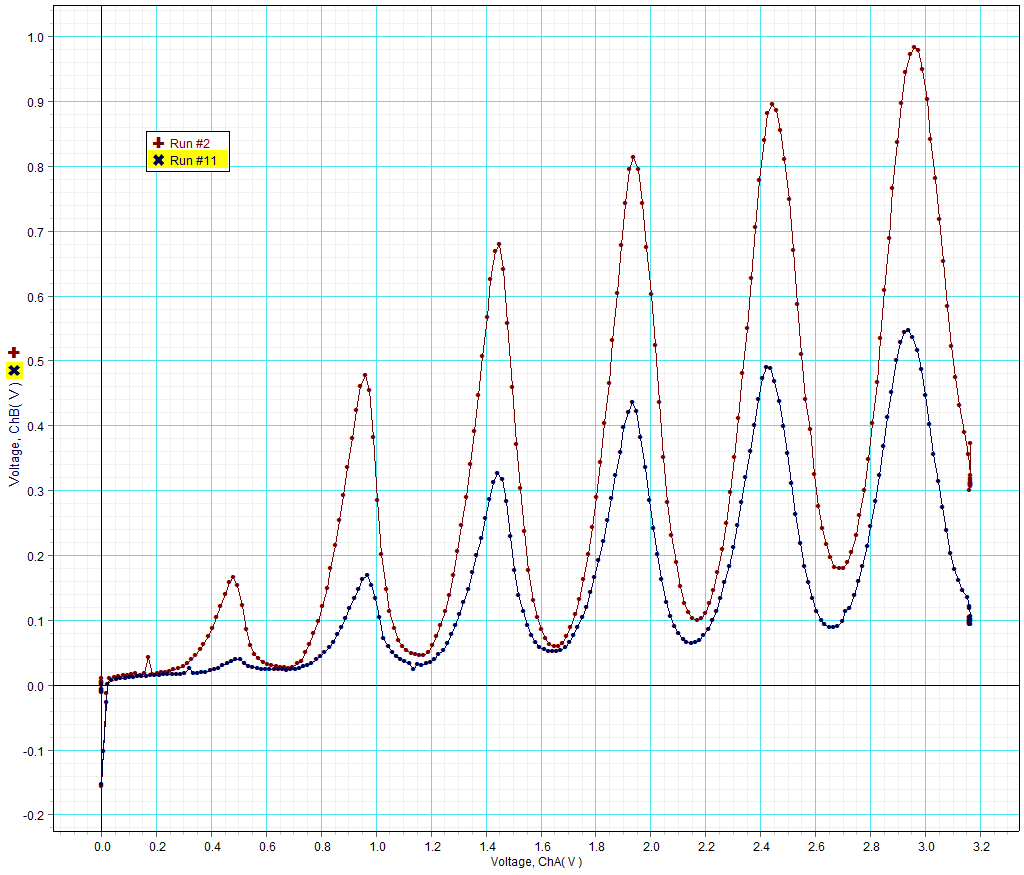
\includegraphics[height=8cm]{scopeoff.png}
        \caption{NoScope!}
    \end{minipage}
    %
    \begin{minipage}{0.37\textwidth}
        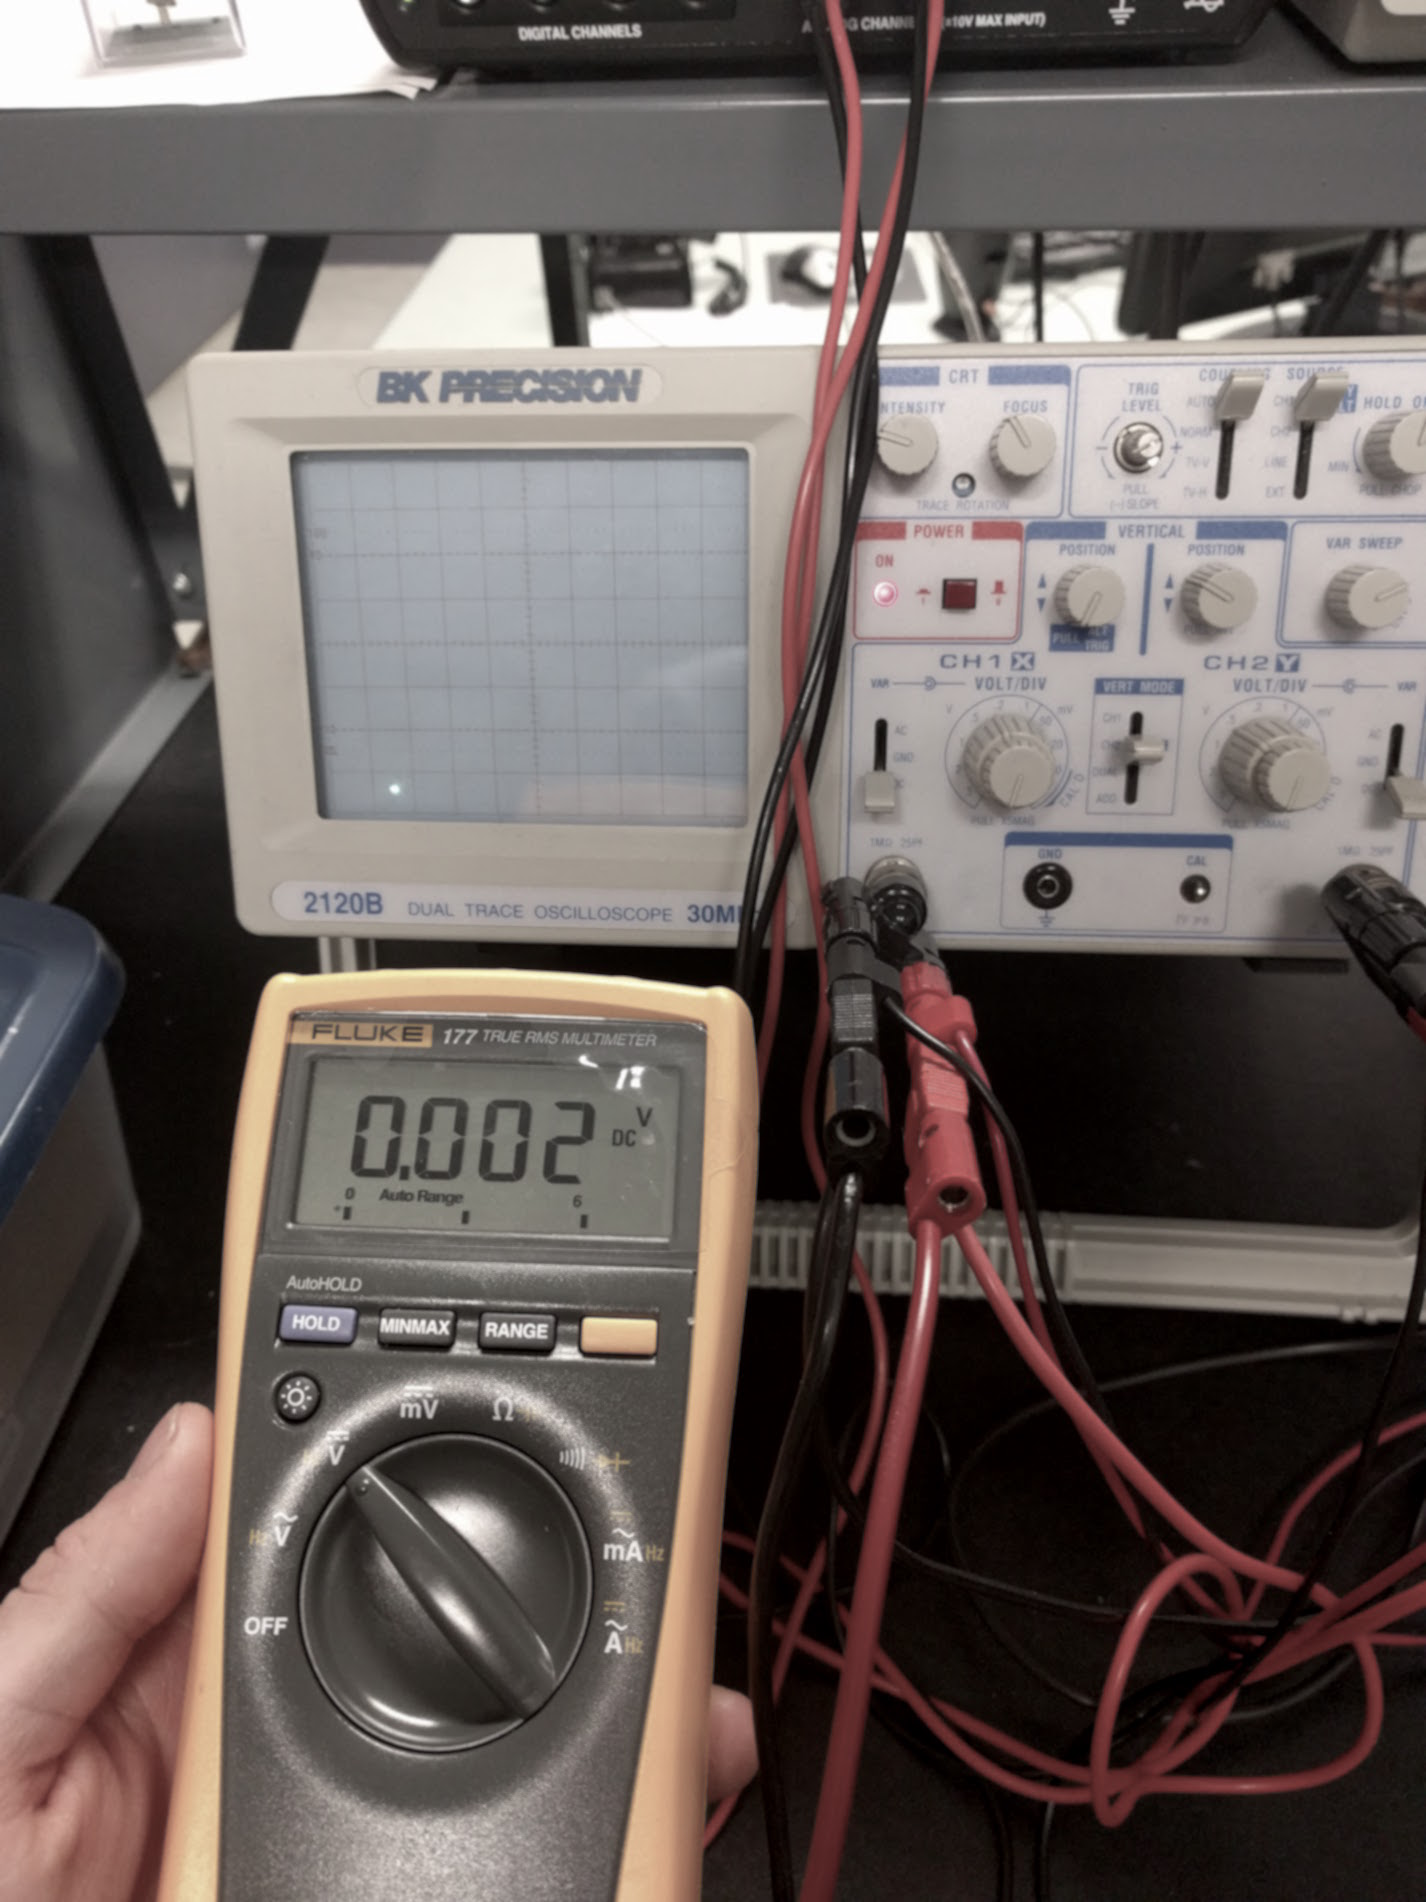
\includegraphics[height=8cm]{voltagedrop.jpg}
        \caption{Voltage Dropped}
    \end{minipage}
\end{figure}

You'll see that this was again confirmed when I probed the oscilloscope terminals with a multimeter with the Frank-Hertz powered down, and found a voltage drop of effectively zero, as shown in the photo below:

\begin{figure}[H]

\end{figure}

\end{quote}}
\end{enumerate}

\section{Error Analysis}
\paragraph{It's difficult to find sources of error in this experiment, given that my partner and I took no part in the setup, and we were not given values for the precision of any of our devices. Had we been measuring currents, it would be possible that the internal resistances of the wires linking the Frank-Hertz power supply had affected our measurements, but because our experiment deals with changes in voltage, we can rule this out. \\My best guess, dissapointingly, is that our main source of error in this experiment was linked to the analog to digital converter that we used to gather data, or bugs in the software that we used to analyze it. That being said, all of our measurements in peak position fall within our expected value (4.9V) by a margin of 0.1V. It's meaningless, but I'd say that we can treat that margin as our uncertainty in this experiment. \\ We could have reduced our accrued error by using higher-precision equipment, running more trials, and analyzing our data more throughly. }



\end{document}
t
